\documentclass{article}

\usepackage[colorlinks, urlcolor=blue, linkcolor=red, citecolor=green]{hyperref}
\usepackage{fancyhdr} %设置页眉和页脚的
\usepackage{extramarks} %设置continue那玩意的
\usepackage{amsmath}
\usepackage{amsthm}
\usepackage{amsfonts}
\usepackage{tikz} %画线的
\usepackage[plain]{algorithm}
\usepackage{algpseudocode}
\usepackage{enumerate}

\usetikzlibrary{automata,positioning}

%表
\usepackage{booktabs}
\usepackage{multirow}
\usepackage{array}
\usepackage{caption}
\DeclareCaptionFont{heiti}{\heiti} %还可以定义其他的
\captionsetup{labelsep=space, font={small, bf}, skip=2pt} %space可以改成quad

%图
%*****************图片及其相关设置***************************
\usepackage{graphicx}
\graphicspath{{tupian/}}
\usepackage{subfigure}
%

%*****************代码相关设置***************************
\usepackage{pythonhighlight}

\usepackage{dsfont}
% Basic Document Settings
%

\topmargin=-0.45in
\evensidemargin=0in
\oddsidemargin=0in
\textwidth=6.5in
\textheight=9.0in
\headsep=0.25in

\linespread{1.1}

\pagestyle{fancy}
\lhead{\hmwkAuthorName}
\chead{\hmwkClass: \hmwkTitle}
\rhead{\firstxmark}
\lfoot{\lastxmark}
\cfoot{\thepage}

\renewcommand\headrulewidth{0.4pt}
\renewcommand\footrulewidth{0.4pt}

\setlength\parindent{0pt}

%
% Create Problem Sections
%

\newcommand{\enterProblemHeader}[1]{
    \nobreak\extramarks{}{Assignment A5.\arabic{#1} continued on next page\ldots}\nobreak{}
    \nobreak\extramarks{Assignment A5.\arabic{#1} (continued)}{Assignment A5.\arabic{#1} continued on next page\ldots}\nobreak{}
}

\newcommand{\exitProblemHeader}[1]{
    \nobreak\extramarks{Assignment A5.\arabic{#1} (continued)}{Assignment A5.\arabic{#1} continued on next page\ldots}\nobreak{}
    \stepcounter{#1}
    \nobreak\extramarks{Assignment A5.\arabic{#1}}{}\nobreak{}
}

\setcounter{secnumdepth}{0}
\newcounter{partCounter}
\newcounter{homeworkProblemCounter}
\setcounter{homeworkProblemCounter}{1}
\nobreak\extramarks{Assignment A5.\arabic{homeworkProblemCounter}}{}\nobreak{}

\newenvironment{homeworkProblem}{
    \section{Assignment A5.\arabic{homeworkProblemCounter}}
    \setcounter{partCounter}{1}
    \enterProblemHeader{homeworkProblemCounter}
}{
    \exitProblemHeader{homeworkProblemCounter}
}

%
% Homework Details
%   - Title
%   - Due date
%   - Class
%   - Section/Time
%   - Instructor
%   - Author
%

\newcommand{\hmwkTitle}{Homework\ \#5}
\newcommand{\hmwkDueDate}{December 28, 2020}
\newcommand{\hmwkClass}{Introduction to Optimization}
\newcommand{\hmwkClassTime}{}
\newcommand{\hmwkClassInstructor}{Professor Andre Milzarek}
\newcommand{\hmwkAuthorName}{Peng Deng}
\newcommand{\hmwkAuthorSchool}{School of Data Science}
\newcommand{\hmwkAuthorNumber}{Sno.220041042}
%
% Title Page
%

\title{
    \vspace{2in}
    \textmd{\textbf{\hmwkClass:\ \hmwkTitle}}\\
    \normalsize\vspace{0.1in}\small{Due\ on\ \hmwkDueDate}\\
    \vspace{0.1in}\large{\textit{\hmwkClassInstructor\ \hmwkClassTime}}
    \vspace{3in}
}

\author{\textbf{\hmwkAuthorName}}

\date{}

\renewcommand{\part}[1]{\textbf{\large Part \Alph{partCounter}}\stepcounter{partCounter}\\}

%
% Various Helper Commands
%

% Useful for algorithms
\newcommand{\alg}[1]{\textsc{\bfseries \footnotesize #1}}

% For derivatives
\newcommand{\deriv}[1]{\frac{\mathrm{d}}{\mathrm{d}x} (#1)}

% For partial derivatives
\newcommand{\pderiv}[2]{\frac{\partial}{\partial #1} (#2)}

% Integral dx
\newcommand{\dx}{\mathrm{d}x}

% Alias for the Solution section header
\newcommand{\solution}{\textbf{\large Solution}}

% Probability commands: Expectation, Variance, Covariance, Bias
\newcommand{\E}{\mathrm{E}}
\newcommand{\Var}{\mathrm{Var}}
\newcommand{\Cov}{\mathrm{Cov}}
\newcommand{\Bias}{\mathrm{Bias}}
\begin{document}

\maketitle
\thispagestyle{empty}

\newpage
\setcounter{page}{1}

\begin{homeworkProblem}
Consider the nonlinear optimization problem
$$
\min _{x \in \mathbb{R}^{2}} f(x):=\left(x_{1}+1\right)^{3}+2\left(x_{2}-x_{1}\right)+\left(x_{2}+1\right)^{2} \quad \text { s.t. } \quad g(x) \leq 0
$$
where the constraint function $g: \mathbb{R}^{2} \rightarrow \mathbb{R}^{3}$ is given by
$$
g_{1}(x):=\left(x_{1}+1\right)^{2}+x_{2}^{2}-4, \quad g_{2}(x):=x_{1}+1, \quad g_{3}(x):=x_{2}
$$
Let us further set $\bar{x}:=(-1,-2)^{\top}$.
\begin{enumerate}[\quad a)]
	\item Sketch the feasible set $X:=\left\{x \in \mathbb{R}^{2}: g(x) \leq 0\right\}$.
	\item Determine the active set $\mathcal{A}(\bar{x})$ and show that $\bar{x}$ is a regular point.
	\item Investigate whether $\bar{x}$ is a KKT point of problem (1) and calculate a corresponding Lagrange multiplier $\bar{\lambda} \in \mathbb{R}^{3}$
	\item Compute the associated critical cone $\mathcal{C}(\bar{x})$ and simplify as far as possible.
	\item Investigate whether $\bar{x}$ is a local solution of problem (1) and explain your answer.
\end{enumerate}

\vspace{4pt}
\textbf{\large{Solution}}

\vspace{4pt}
\textbf{Subproblem (a)}

As we can see from Figure \ref{seta}, the yellow area is corresponded to $g_1(x)\le 0$, the purple area is corresponded to $g_2(x)\le0$, the green area is corresponded to $g_3(x)\le0$. Thus, the intersection of the three areas is corresponded to $g(x) \le 0$.
\begin{figure}[htbp]
	\centering
	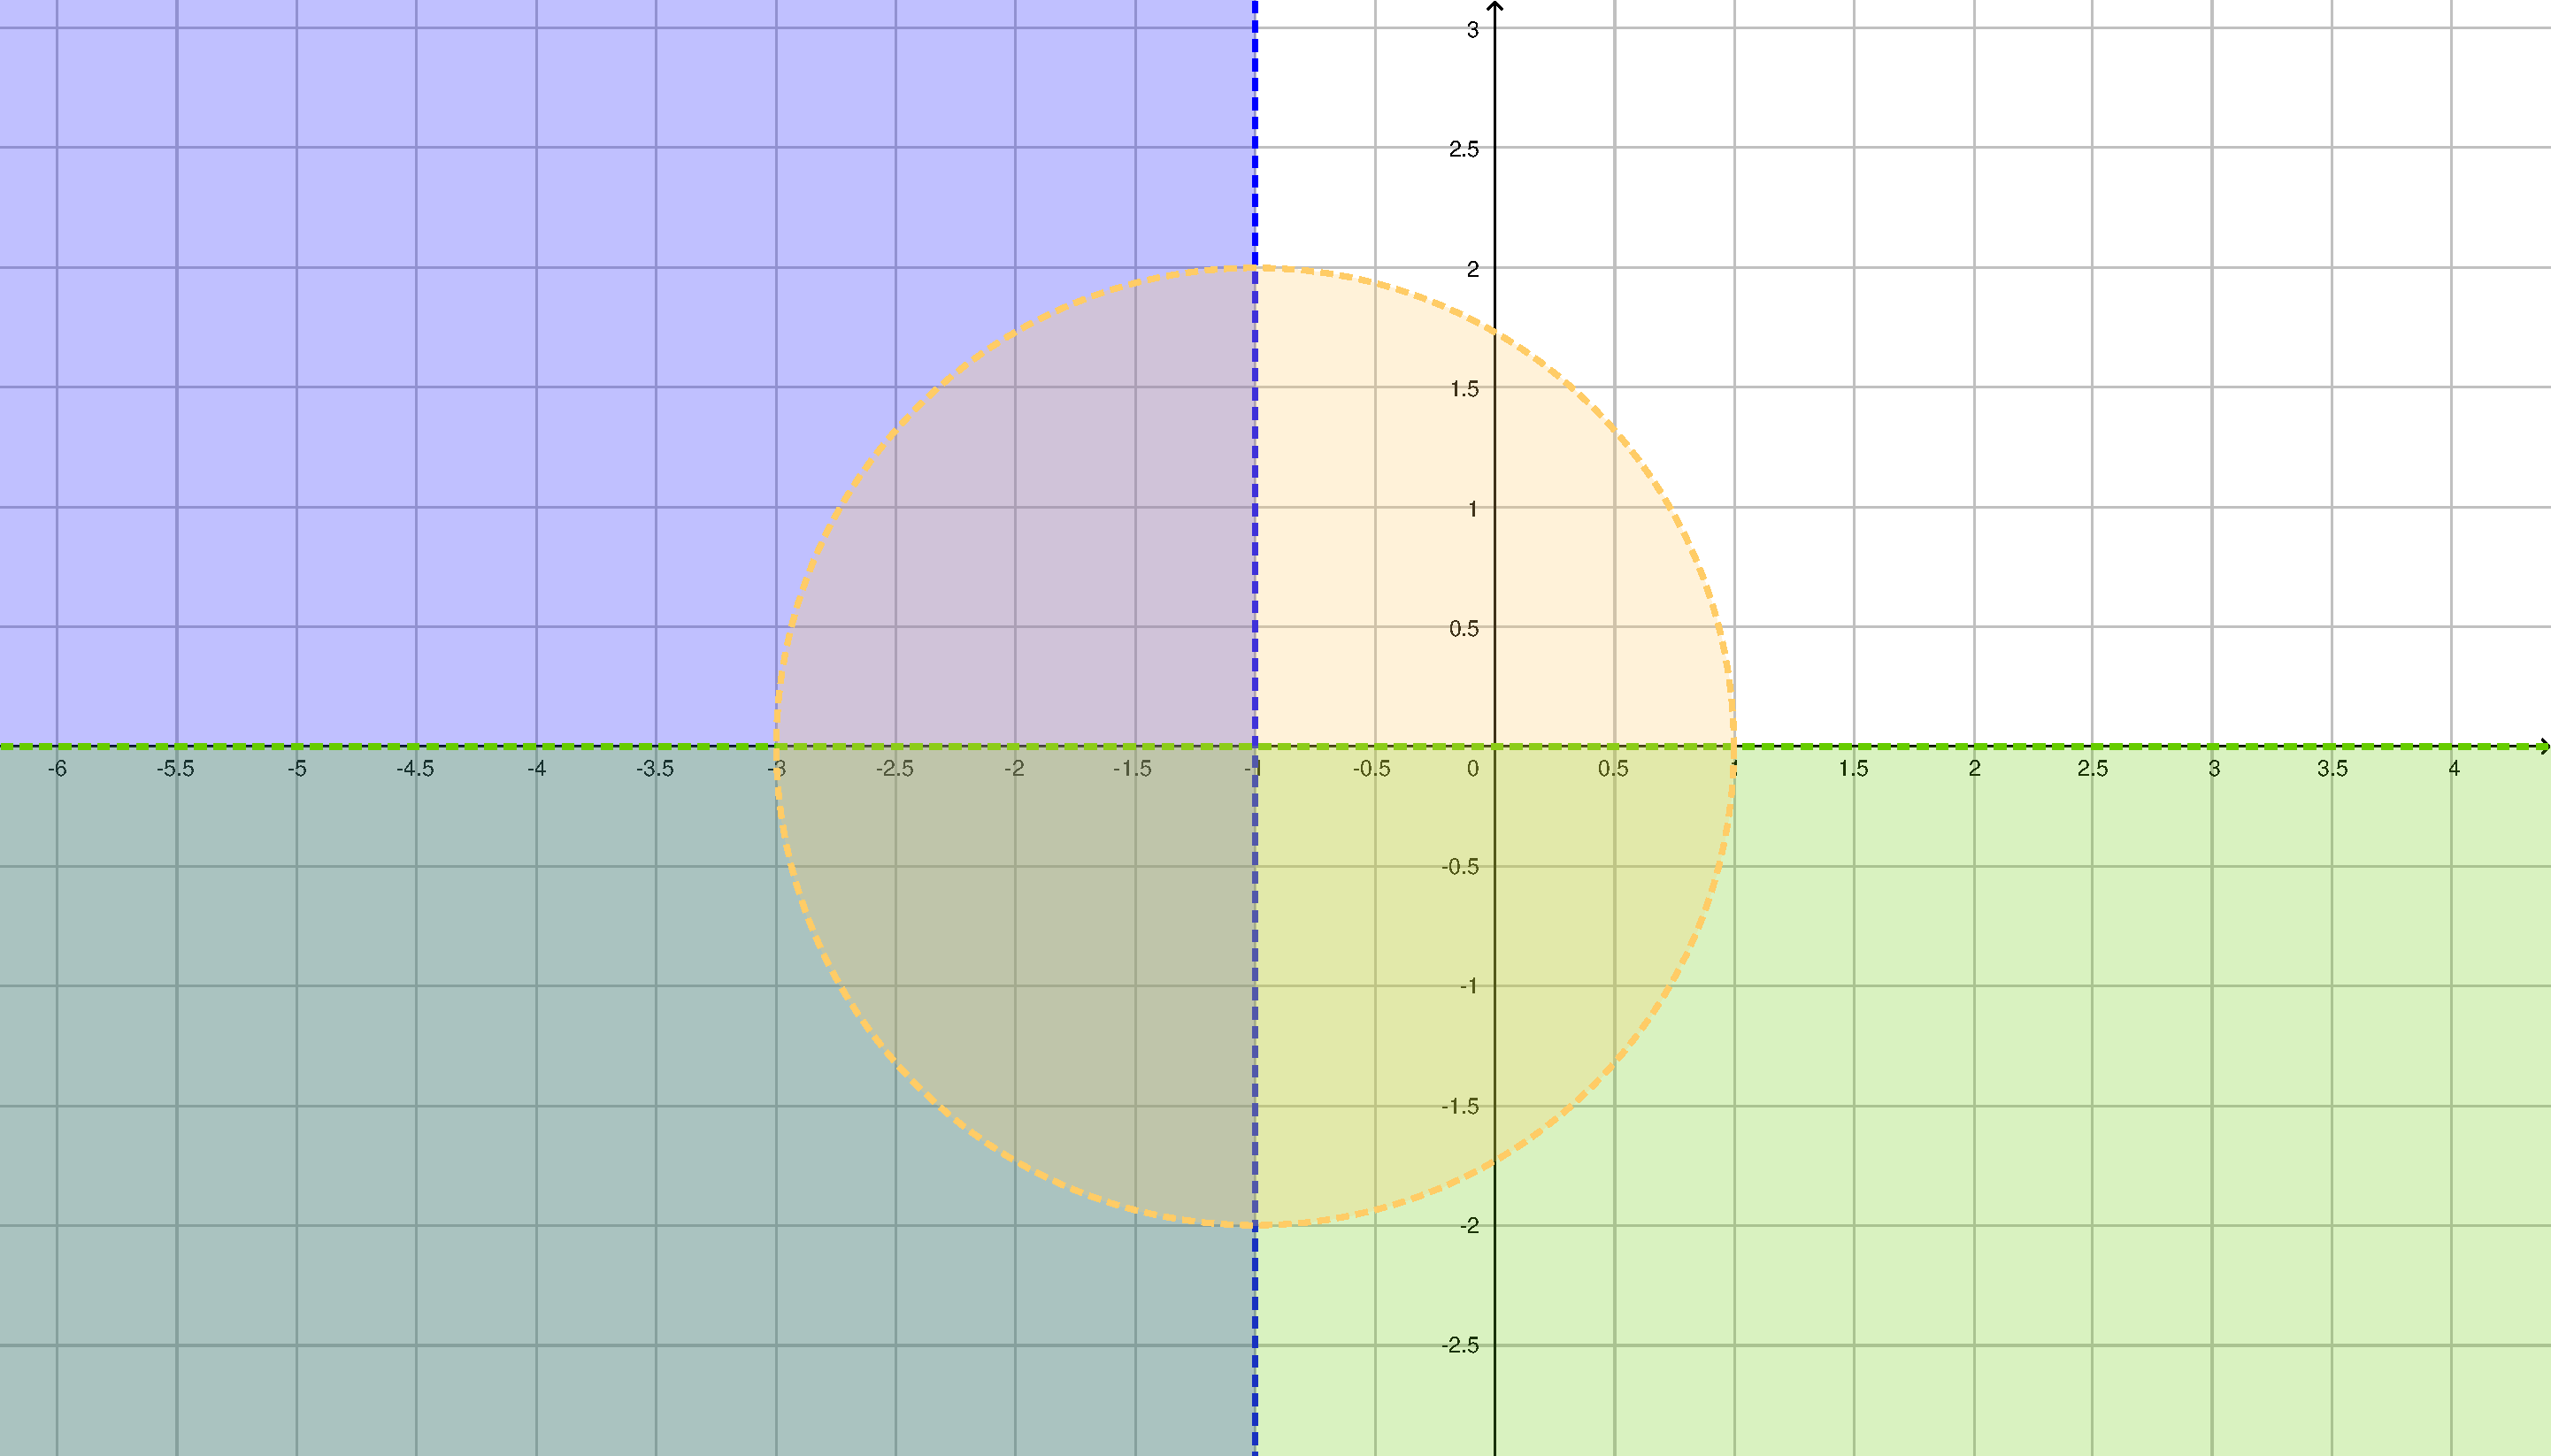
\includegraphics[width=0.7\linewidth]{A5.1_a}
	\vspace{5pt}
	\caption{The feasible set \textbf{\textit{X}}}
	\label{seta}
\end{figure}

\vspace{4pt}
\textbf{Subproblem (b)}

$\circ$ $\bar{x}:=(-1,-2)^{\top}$, so we have 
\begin{equation}
	\begin{split}
		g_{1}(\bar{x})&=\left(-1+1\right)^{2}+(-2)^{2}-4=0\\
		g_{2}(\bar{x})&=x_{1}+1=-1+1=0\\
		g_{3}(\bar{x})&=x_{2}=-2
	\end{split}
\end{equation}
Thus, we can get $\mathcal{A}(\bar{x}) = \left\{1,2\right\}$.

$\circ$ In order to show that $\bar{x}$ is a regular point, we have to show that $\bar{x}$ is a feasible set and satisfy the LICQ. Firstly, it is easy to find that $\bar{x}$ is a feasible point. Then, we have to prove that it satisfies the LICQ. We have
\begin{equation}
	\begin{split}
		\begin{pmatrix}
			\nabla g_1(\bar{x}) & \nabla g_2(\bar{x})
		\end{pmatrix}
		&=
		\begin{pmatrix}
			\nabla g_1(\bar{x}) & \nabla g_2(\bar{x})
		\end{pmatrix}\\
		&=
		\begin{pmatrix}
			2(x_1 + 1) & 1 \\
			2x_2 & 0 \\
		\end{pmatrix}\\
		& = 
		\begin{pmatrix}
			0 & 1 \\
			-4 & 0 \\
		\end{pmatrix}\\
	\end{split}
\end{equation}
We can see the rank of this matrix is 2, which means the matrix has full rank, so $\nabla g_1(\bar{x})$ and $\nabla g_2(\bar{x})$ are linear independent. Thus, we have proved that $\bar{x}$ satisfies the LICQ. In all, we have showed that $\bar{x}$ is a regular point.

\vspace{4pt}
\textbf{Subproblem (c)}

Firstly, we derive the gradients and Hessian as follow:
\begin{equation}
	\begin{split}
		\nabla f(x) &= 
		\begin{pmatrix}
			3\left(x_1+1\right)^2-2\\
			2x_2+4
		\end{pmatrix}\qquad
		\nabla^2 f(x)=
		\begin{pmatrix}
			6x_1 + 6&0\\
			0&2
		\end{pmatrix}
		\\
		\nabla g_1(x) &= 
		\begin{pmatrix}
			2\left(x_1+1\right)\\
			2x_2
		\end{pmatrix}\qquad
		\nabla^2 g_1(x) = 
		\begin{pmatrix}
			2 & 0\\
			0 & 2
		\end{pmatrix}
		\\
		\nabla g_2(x) &= 
		\begin{pmatrix}
			1\\
			0
		\end{pmatrix}\qquad
		\nabla^2 g_2(x) = 
		\begin{pmatrix}
			0 & 0\\
			0 & 0
		\end{pmatrix}
		\\
		\nabla g_3(x) &=
		\begin{pmatrix}
			0\\
			1
		\end{pmatrix}\qquad
		\nabla^2 g_3(x) = 
		\begin{pmatrix}
			0 & 0\\
			0 & 0
		\end{pmatrix}
		\\
	\end{split}
\end{equation}
Let's check the KKT-conditions. Due to $\mathcal{I}(\bar{x}) = \left\{3\right\}$, we know $\bar{\lambda}_3=0$.

$\circ$ Main Cond:
\begin{equation}
	\begin{split}
		&\nabla f(\bar{x})+\bar{\lambda}_1\nabla g_1(\bar{x}) + \bar{\lambda}_2\nabla g_2(\bar{x}) = 0\\
		\Longrightarrow&
		\begin{pmatrix}
			-2\\
			0
		\end{pmatrix}+\bar{\lambda}_1
		\begin{pmatrix}
			0\\
			-4
		\end{pmatrix}+\bar{\lambda}_2
		\begin{pmatrix}
			1\\
			0
		\end{pmatrix}=0\\
		\Longrightarrow&
		\bar{\lambda}_1 = 0, \quad \bar{\lambda}_2 = 2
	\end{split}
\end{equation}
$\circ$ Dual Feasibility
\begin{equation}
	\begin{split}
	\bar{\lambda}_1 &=0 \ge 0\\
	\bar{\lambda}_2 &=2 \ge 0\\
	\bar{\lambda}_3 &=0 \ge 0
	\end{split}
\end{equation}
$\circ$ Complementarity
\begin{equation}
	\begin{split}
	\bar{\lambda}_1\cdot g_1(\bar{x}) &= 0\\
	\bar{\lambda}_2\cdot g_2(\bar{x}) &= 2\cdot (-1+1) = 0\\
	\bar{\lambda}_3\cdot g_3(\bar{x}) &= 0\\
	\end{split}
\end{equation}
$\circ$ Primal Feasibility
\begin{equation}
	\begin{split}
		g_1(\bar{x})&=0\le 0\\
		g_2(\bar{x})&=0\le 0\\
		g_3(\bar{x})&=-2\le 0\\
	\end{split}
\end{equation}
Thus, $\bar{x}$ is a KKT point. The corresponding Lagrange multiplier $\bar{\lambda}$=$\left(\bar{\lambda}_1,\bar{\lambda}_2 ,\bar{\lambda_3}\right)^{\top}=\left(0, 2, 0\right)^{\top}$.

\vspace{4pt}
\textbf{Subproblem (d)}
\begin{equation}
	\begin{split}
		\mathcal{C}(\bar{x})&=\left\{d\in \mathbb{R}^2:\nabla f(\bar{x})^{\top}d=0,\nabla g_i(\bar{x})^{\top}d\le 0,\forall i\in \mathcal{A}(\bar{x})\right\}\\
		&=\left\{d\in \mathbb{R}^2:
		(-2,0)
		\begin{pmatrix}
			d_1\\
			d_2
		\end{pmatrix}=0;\,\,
		(0, -4)
		\begin{pmatrix}
			d_1\\
			d_2
		\end{pmatrix}\le 0;\,\,
		(1, 0)
		\begin{pmatrix}
			d_1\\
			d_2
		\end{pmatrix}\le 0
		\right\}\\
		&=\left\{d\in \mathbb{R}^2:d_1=0, d_2\ge 0\right\}\\
		&=\left\{(0, t)^{\top}, t\ge 0\right\}\\
	\end{split}
\end{equation}

\vspace{4pt}
\textbf{Subproblem (e)}

In order to investigate whether $\bar{x}$ is a local solution, we need to check whether $\nabla^2_{xx} L\left(\bar{x},\bar{\lambda}\right)$ is positive definite. We have
\begin{equation}
	\begin{split}
		\nabla^2_{xx} L\left(\bar{x},\bar{\lambda}\right) &= \nabla^2f(\bar{x})+\sum_{i=1}^3\lambda_i\nabla^2g_i(\bar{x})\\
		&=\nabla^2f(\bar{x})+\bar{\lambda}_2\nabla^2g_2(\bar{x})\\
		&=
		\begin{pmatrix}
			0&0\\
			0&2
		\end{pmatrix}
		+2\cdot
		\begin{pmatrix}
			0&0\\
			0&0
		\end{pmatrix}\\
		&=
		\begin{pmatrix}
			0&0\\
			0&2
		\end{pmatrix}
	\end{split}
\end{equation}
Then we can get
\begin{equation}
	d^{\top} \nabla^2_{xx} L\left(\bar{x},\bar{\lambda}\right) d=
	(0,t)
	\begin{pmatrix}
		0&0\\
		0&2
	\end{pmatrix}
	\begin{pmatrix}
		0\\t
	\end{pmatrix}=2t^2
\end{equation}
So we have $d^{\top} \nabla^2_{xx} L\left(\bar{x},\bar{\lambda}\right) d > 0$ for all $d\in \mathcal{C}(\bar{x})\backslash \{0\}$. $\nabla^2_{xx} L\left(\bar{x},\bar{\lambda}\right)$ is positive definite on $\mathcal{C}(\bar{x})$. Thus, we can conclude that $\bar{x}$ is a local solution.
\end{homeworkProblem}

\begin{homeworkProblem}
Let $n \in \mathbb{N}$ be given. Let us consider the problem
$$
\min _{x \in \mathbb{R}^{n}} f(x)=\sum_{j=1}^{n} x_{j}^{j} \quad \text { s.t. } \quad g(x)=1-\|x\|_{2}^{2} \leq 0
$$
and let $X:=\left\{x \in \mathbb{R}^{n}: g(x) \leq 0\right\}$ denote the corresponding feasible set.
\begin{enumerate}[\quad a)]
	\item Show that the LICQ is satisfied at every feasible point of (2) .
	\item Verify that the point $\bar{x}=(1,0,0, \ldots, 0)^{\top} \in \mathbb{R}^{n}$ and the multiplier $\bar{\lambda}=\frac{1}{2}$ form a KKT pair of problem (2)
	\item Compute the critical cone $\mathcal{C}(\bar{x})$ and simplify as far as possible.
	\item Apply the second-order necessary and sufficient conditions and show that $\bar{x}$ is a local solution of problem (2) if and only if $n \leq 2$.
\end{enumerate}

\vspace{4pt}
\textbf{Subproblem (a)}

In order to show that LICQ satisfied at every point, we have to show that the vector set $\left\{\nabla g_i(\bar{x}): i\in \mathcal{A}(\bar{x})\right\}$ is linearly independent. We have
\begin{equation}
	\nabla g(\bar{x}) = \left(-2\bar{x}_1,-2\bar{x}_2,\dots,-2\bar{x}_n\right)^{\top}
\end{equation}
When $g(\bar{x}) < 0$, the active set $\mathcal{A}(\bar{x})$ is empty, so the LICQ is satisfied automatically at this point. When $g(\bar{x}) = 0$, the active set $\mathcal{A}(\bar{x})=\left\{1\right\}$. So we have to prove $\left\{\nabla g_1(\bar{x})\right\}$ is linearly independent. We have
\begin{equation}
	\begin{split}
		&g(\bar{x}) = 0\\
		\Longrightarrow&\|\bar{x}\|_2^2=1
	\end{split}
\end{equation}
Thus, $\bar{x} \ne 0$, which means $\bar{x}_1, \bar{x}_2, \dots ,\bar{x}_n$ can not equal 0 simultaneously. So we can derive that $\nabla g_1(\bar{x})\ne 0$, so the vector set $\left\{\nabla g_1(\bar{x})\right\}$ is linearly independent.

Above all, we have showed thta LICQ is satisfied at every feasible point.

\vspace{4pt}
\textbf{Subproblem (b)}

Firstly, we derive the gradients and Hessian as follow:
\begin{equation}
	\begin{split}
		\nabla f(x) &= 
		\begin{pmatrix}
			1\\
			2x_2\\
			3x_3^2\\
			\vdots\\
			nx_n^{n-1}
		\end{pmatrix}\qquad
		\nabla^2f(x)=
		\begin{pmatrix}
			0&0&0&\cdots &0\\
			0&2&0&\cdots &0\\
			0&0&6x_3&\cdots&0\\
			\vdots&\vdots&\vdots&\ddots&\vdots\\
			0&0&0&\cdots&n(n-1)x_n^{n-2}
		\end{pmatrix}\\
		\nabla g(x) &= 
		\begin{pmatrix}
			-2x_1\\
			-2x_2\\
			-2x_3\\
			\vdots\\
			-2x_n
		\end{pmatrix}\qquad
		\nabla ^2 g(x) = 
		\begin{pmatrix}
			-2&0&0&\cdots &0\\
			0&-2&0&\cdots &0\\
			0&0&-2&\cdots&0\\
			\vdots&\vdots&\vdots&\ddots&\vdots\\
			0&0&0&\cdots&-2
		\end{pmatrix}\\
	\end{split}
\end{equation}
Let's check the KKT-conditions. We have $g(\bar{x})=0$, so $\mathcal{A}(x)=\left\{1\right\}$.

$\circ$ Main Cond:
\begin{equation}
	\nabla f(\bar{x}) + \bar{\lambda}\nabla g(\bar{x}) =
	\begin{pmatrix}
		1\\0\\0\\ \vdots\\ 0
	\end{pmatrix} + \bar{\lambda}\cdot
	\begin{pmatrix}
		-2\\0\\0\\ \vdots\\ 0
	\end{pmatrix}=
	\begin{pmatrix}
		1\\0\\0\\ \vdots\\ 0
	\end{pmatrix} + \frac{1}{2}\cdot
	\begin{pmatrix}
		-2\\0\\0\\ \vdots\\ 0
	\end{pmatrix}=0
\end{equation}
$\circ$ Dual Feasibility
\begin{equation}
	\bar{\lambda} = \frac{1}{2} \ge 0
\end{equation}
$\circ$ Complemenrarity
\begin{equation}
	\bar{\lambda}\cdot g(\bar{x}) = \frac{1}{2} \cdot 0 = 0
\end{equation}
$\circ$ Primal Feasibility
\begin{equation}
	g(\bar{x}) = 0 \le 0
\end{equation}
Thus, the point $\bar{x}$ satisfied the KKT conditions with $\bar{\lambda} = \frac{1}{2}$, and it is easy to find that $\bar{x}$ is a feasible point. 

Above all,  we have verified that the point $\bar{x}$ and the multiploer $\bar{\lambda}$ from a KKT pair.

\vspace{4pt}
\textbf{Subproblem (c)}
\begin{equation}
	\begin{split}
		\mathcal{C}(\bar{x})&=\left\{d\in \mathbb{R}^n:\nabla f(\bar{x})^{\top}d=0,\nabla g_i(\bar{x})^{\top}d\le 0,\forall i\in \mathcal{A}(\bar{x})\right\}\\
		&=\left\{d\in \mathbb{R}^n:
		(1,0,0,\cdots, 0)
		\begin{pmatrix}
			d_1\\
			d_2\\
			d_3\\
			\vdots\\
			d_n
		\end{pmatrix}=0;\,\,
		(-2, 0,0,\cdots, 0)
		\begin{pmatrix}
			d_1\\
			d_2\\
			d_3\\
			\vdots\\
			d_n
		\end{pmatrix}\le 0\right\}\\
		&=\left\{d\in \mathbb{R}^n:d_1=0\right\}\\
	\end{split}
\end{equation}

\vspace{4pt}
\textbf{Subproblem (d)}

In order to investigate whether $\bar{x}$ is a local solution, we need to check whether $\nabla^2_{xx} L\left(\bar{x},\bar{\lambda}\right)$ is positive definite. We have
\begin{equation}
	\begin{split}
		\nabla^2_{xx} L\left(\bar{x},\bar{\lambda}\right) &= \nabla^2f(\bar{x})+ \bar{\lambda}\nabla^2g(\bar{x})\\
		&=
		\begin{pmatrix}
			0&0&0&\cdots &0\\
			0&2&0&\cdots&0\\
			0&0&0&\cdots &0\\
			\vdots&\vdots&\vdots&\ddots &\vdots\\
			0&0&0&\cdots &0\\
		\end{pmatrix}
		+\frac{1}{2}\cdot
		\begin{pmatrix}
			-2&0&0&\cdots &0\\
			0&-2&0&\cdots&0\\
			0&0&-2&\cdots &0\\
			\vdots&\vdots&\vdots&\ddots &\vdots\\
			0&0&0&\cdots &-2\\
		\end{pmatrix}\\
		&=
		\begin{pmatrix}
			-1&0&0&\cdots &0\\
			0&1&0&\cdots&0\\
			0&0&-1&\cdots &0\\
			\vdots&\vdots&\vdots&\ddots &\vdots\\
			0&0&0&\cdots &-1\\
		\end{pmatrix}
	\end{split}
\end{equation}
$\circ$ When $n=1$, we have
\begin{equation}
	d^{\top} \nabla^2_{xx} L\left(\bar{x},\bar{\lambda}\right) d=
	(0)
	\begin{pmatrix}
		-1
	\end{pmatrix}
	\begin{pmatrix}
		0
	\end{pmatrix}=0
\end{equation}
We can see $\mathcal{C}(\bar{x})=\left\{(0)\right\}$ in this situation. Thus, $\nabla^2_{xx} L\left(\bar{x},\bar{\lambda}\right)$ is positive definite on $\mathcal{C}(\bar{x})$. Thus, $\bar{x}$ is a local solution.

$\circ$ When $n=2$, we have $\mathcal{C}(\bar{x})=\left\{(0, d_2)^{\top}\right\}$
\begin{equation}
	d^{\top} \nabla^2_{xx} L\left(\bar{x},\bar{\lambda}\right) d=
	(0,d_2)
	\begin{pmatrix}
		-1&0\\0&1
	\end{pmatrix}
	\begin{pmatrix}
		0\\d_2
	\end{pmatrix}=d_2^2
\end{equation}
So we have $d^{\top} \nabla^2_{xx} L\left(\bar{x},\bar{\lambda}\right) d > 0 $ for all $d\in \mathcal{C}(\bar{x})\backslash\left\{0\right\}$. $\nabla^2_{xx} L\left(\bar{x},\bar{\lambda}\right)$ is positive definite on $\mathcal{C}(\bar{x})$. Thus, $\bar{x}$ is a local solution.

$\circ$ When $n\ge3$, we have $\mathcal{C}(\bar{x})=\left\{(0, d_2, d_3, \cdots, d_n)^{\top}\right\}$
\begin{equation}
	d^{\top} \nabla^2_{xx} L\left(\bar{x},\bar{\lambda}\right) d=
	(0,d_2,  d_3, \cdots, d_n)
	\begin{pmatrix}
		-1&0&0&\cdots &0\\
		0&1&0&\cdots&0\\
		0&0&-1&\cdots &0\\
		\vdots&\vdots&\vdots&\ddots &\vdots\\
		0&0&0&\cdots &-1\\
	\end{pmatrix}
	\begin{pmatrix}
		0\\d_2\\d_3\\ \cdots\\d_n
	\end{pmatrix}=d_2^2-\sum_{i=3}^{n}d_i^2
\end{equation}
Because $d_i$ is arbitrary for all $i\ge 2$, so we do not have $d^{\top} \nabla^2_{xx} L\left(\bar{x},\bar{\lambda}\right) d > 0 $ for all $d\in \mathcal{A}(\bar{x})\backslash\left\{0\right\}$, which means $\nabla^2_{xx} L\left(\bar{x},\bar{\lambda}\right)$ is not positive definite on $\mathcal{C}(\bar{x})$. Thus, $\bar{x}$ is not local solution.
\end{homeworkProblem}

\begin{homeworkProblem}
Let $a \in \mathbb{R}^{n} \backslash\{0\}$ and $b \in \mathbb{R}$ be given and define the set $C:=\left\{x \in \mathbb{R}^{n}: a^{\top} x \leq b\right\} .$ Compute the projection $\mathcal{P}_{C}(x)$ for $x \in \mathbb{R}^{n},$ i.e., solve the optimization problem
$$
\min _{y \in \mathbb{R}^{n}} \frac{1}{2}\|y-x\|^{2} \quad \text { s.t. } \quad a^{\top} y \leq b
$$

We have
\begin{equation}
	\begin{split}
		f(y) &= \frac{1}{2}\|y-x\|^2\qquad \nabla f(y) = y-x\\
		g(y) &=a^{\top}y-b\le 0\qquad \nabla g(y) = a
	\end{split}
\end{equation}
We apply KKT condition as follow, suppose $y^*$ is the solution.

$\circ$ Main Cond
\begin{equation}
	\label{eq24}
	\begin{split}
		\nabla f(y^*) + \lambda \nabla g(y^*) &= y^*-x + \lambda\cdot a = 0
	\end{split}
\end{equation}
$\circ$ Dual Feasibility
\begin{equation}
	\lambda \ge 0
\end{equation}
$\circ$ Complementarity
\begin{equation}
	\label{eq26}
	\lambda\cdot g(y^*) =0
\end{equation}
$\circ$ Primal Feasibility
\begin{equation}
	\label{eq27}
	g(y^*) \le 0
\end{equation}
$\bullet$ Case 1: $a^{\top}y^*< b$, which means $g(y^*) < 0$

Due to equation \ref{eq26}, we can have $\lambda=0$. Due to equation \ref{eq24}, we can have $y^* = x$. Due to $a^{\top}y^*< b$ and  $y^* = x$, we can get $a^{\top}x< b$. Thus, when $a^{\top}x< b$, we have $y^* = x$.

$\bullet$ Case 2: $a^{\top}y^*= b$, which means $g(y^*) = 0$

In this situation, Complementarity is satisfied. And we have
\begin{equation}
	\label{eq28}
	\begin{split}
		&g(y^*) = 0\\
		\Longrightarrow & a^{\top} y^* = b
	\end{split}
\end{equation}
Combine the equation \ref{eq24} and equation \ref{eq28}, we can get
\begin{equation}
	\begin{split}
		\lambda &= \frac{a^{\top}x-b}{a^{\top}a}\\
		y^*&= x - \frac{a^{\top}x-b}{a^{\top}a}\cdot a
	\end{split}
\end{equation}
In this situation, the $\lambda$ should satisfy $\lambda \ge 0$. So
\begin{equation}
	\begin{split}
		&\lambda = \frac{a^{\top}x-b}{a^{\top}a}\ge 0\\
		\Longrightarrow&a^{\top}x\ge b
	\end{split}
\end{equation}
Thus, when $a^{\top}x\ge b$, we have $y^* = x - \left(a^{\top}x-b\right)\cdot\left(a^{\top}a\right)^{-1}\cdot a$. 

It is easy to show that the function $f(y)$ is convex. Because $g(x) = x^2,(x\in \mathbb{R})$ is convex and non-decreasing. Besides, $h(x) = \|x\|, (x\in \mathbb{R}^n)$ is convex. So the composition $g(h(x))$ is convex, so $f(y)$ is convex. On the other hand, the set $\left\{y\in\mathbb{R}^n:a^{\top}y\le b\right\}$ is a half space, so it is convex. Overall, the problem is a convex optimization problem. So the KKT-point $y^*$ is a global solution.

Thus we have derived the projection
\begin{equation}
	\mathcal{P}_C(x) = 
	\begin{cases}
		x & \left(a^{\top}x< b\right)\\
		x - \left(a^{\top}x-b\right)\cdot\left(a^{\top}a\right)^{-1}\cdot a&\left(a^{\top}x\ge b\right)
	\end{cases}
\end{equation}
\end{homeworkProblem}

\end{document}

